\documentclass{article}

\usepackage{graphicx}
\usepackage{tikz}
\usepackage{tikzsymbols}
\usetikzlibrary{calc,patterns,shapes.geometric}
\pagestyle{empty}
\usepackage[margin=0pt]{geometry}
\geometry{papersize={14in,12in}}

\def\centerarc[#1](#2)(#3:#4:#5){\draw[#1] ($(#2)+({#5*cos(#3)},{#5*sin(#3)})$) arc (#3:#4:#5);}

\begin{document}
	\begin{figure}
		\centering
		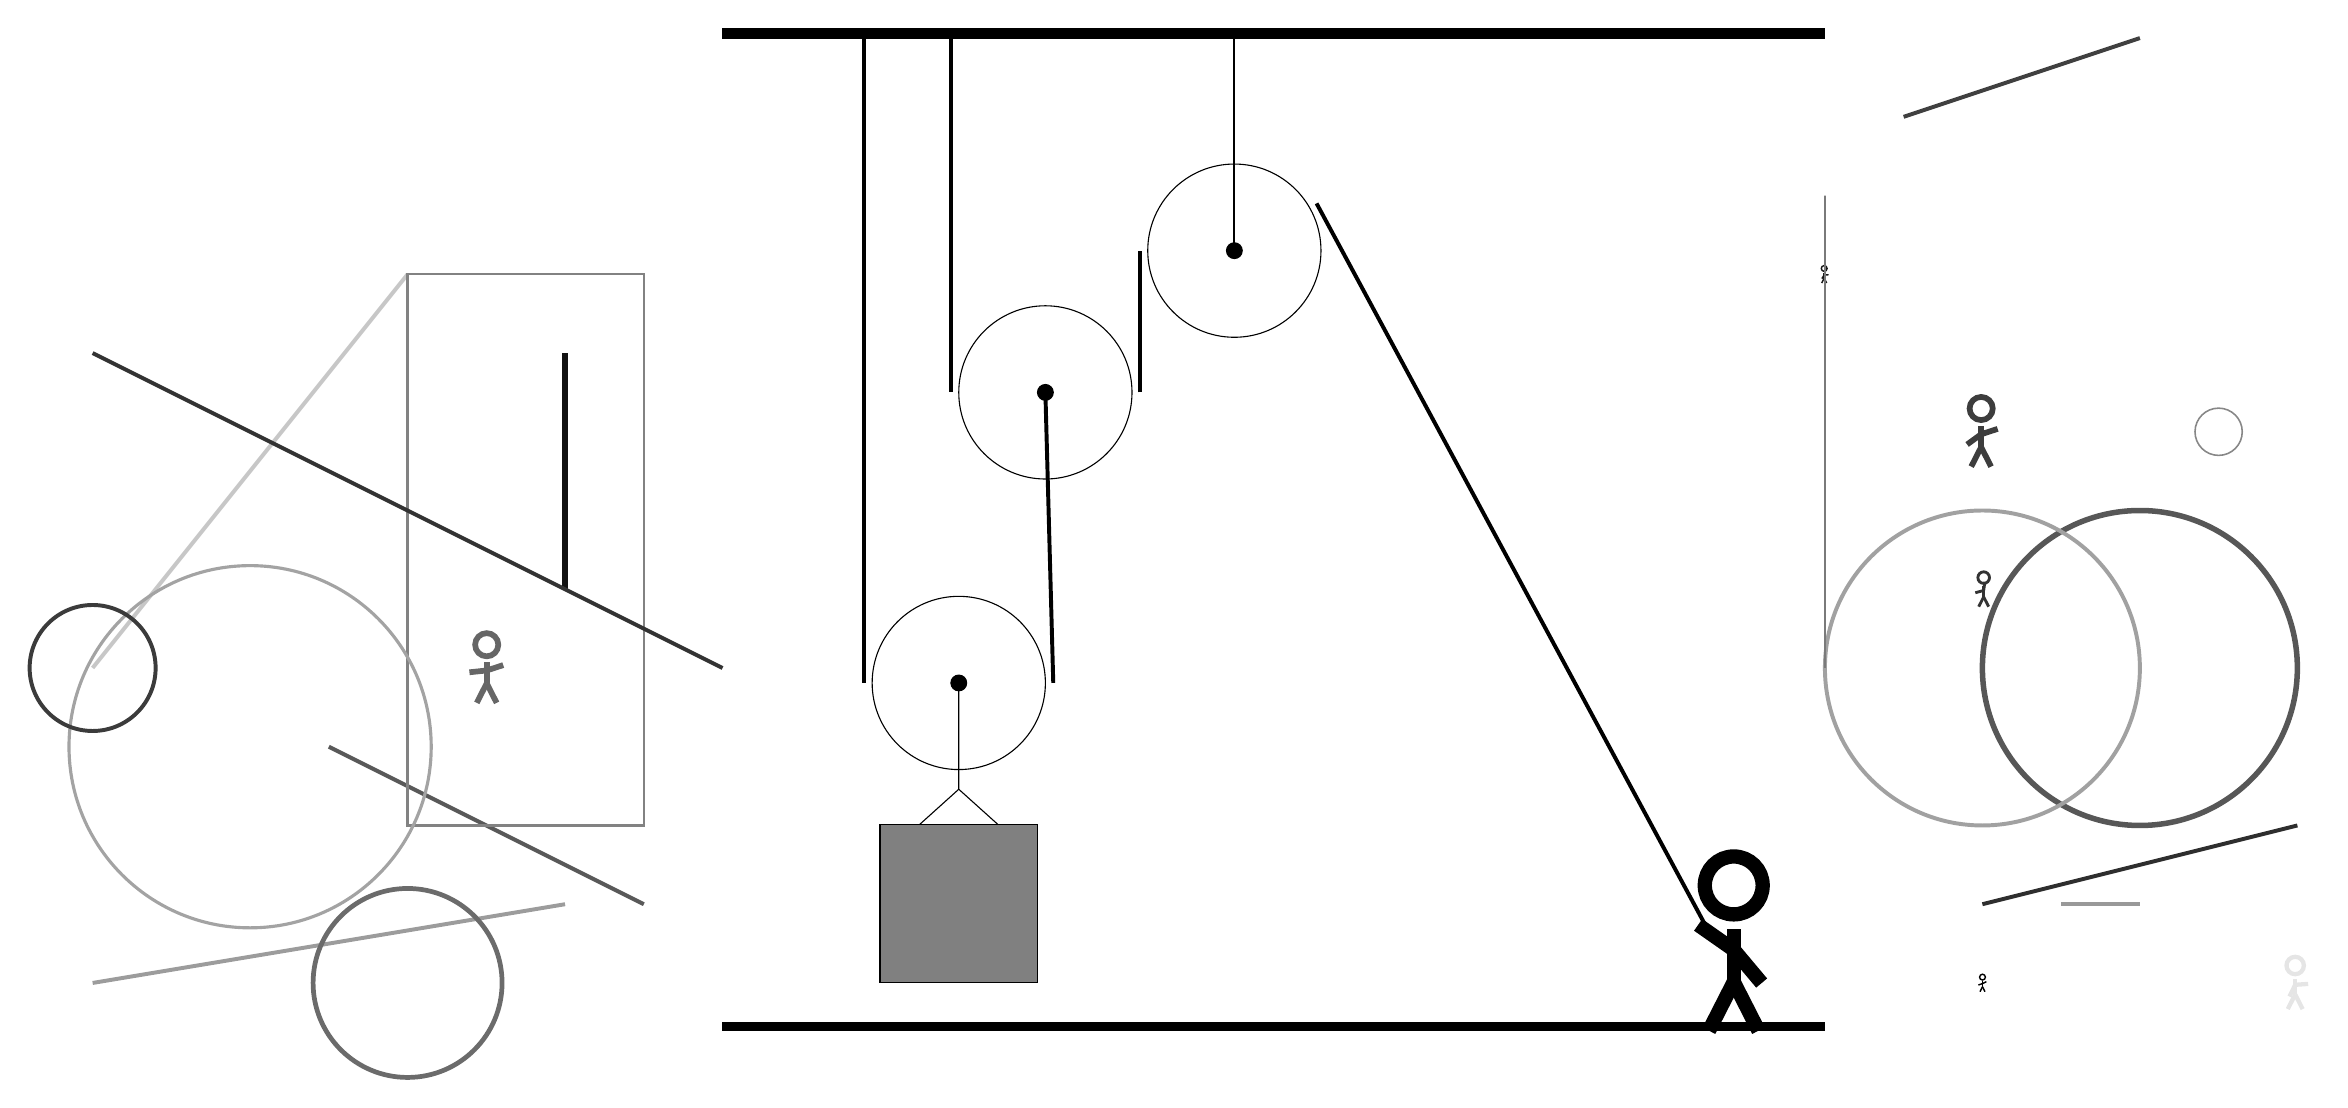
\begin{tikzpicture}
			%%%%% START %%%%%
			
			\draw[fill=black] (-2, 9) rectangle (12, 9.125);
			
			\draw (1, 0.81) circle (1.1);
			\draw[fill=black] (1, 0.81) circle (0.1);
			
			\draw (2.1, 4.5) circle (1.1);
			\draw[fill=black] (2.1, 4.5) circle (0.1);
			
			\draw (4.5, 6.3) circle (1.1);
			\draw[fill=black] (4.5, 6.3) circle (0.1);
			\draw[thick] (4.5, 6.3) -- (4.5, 9);
			
			\draw (1, 0.81) -- (1, -0.54) -- (0.5, -0.99) -- (1.5, -0.99) -- (1, -0.54);
			\draw[fill=black!50] (0, -0.99) rectangle (2, -2.99);
			
			\node[line width=0.6mm, color=black!91] at (12, 6) {\Strichmaxerl[1][58][2]};
			
			\node[line width=0.2mm, color=black!99] at (14, -3) {\Strichmaxerl[1][19][26]};
			\draw [line width=0.7mm, color=black!66](16, 1) circle (2.0);
			\draw[line width=0.5mm, color=black!75](13, 8) -- (16, 9);
			\draw[line width=0.5mm, color=black!22](-6, 6) -- (-10, 1);
			\node[line width=0.5mm, color=black!10] at (18, -3) {\Strichmaxerl[3][64][4]};
			
			\draw[line width=0.5mm, color=black!65](-7, 0) -- (-3, -2);
			\draw[line width=0.3mm, color=black!49] (-3, -1) rectangle (-6, 6);
			\draw [line width=0.5mm, color=black!37](14, 1) circle (2.0);
			\node[line width=0.4mm, color=black!60] at (-5, 1) {\Strichmaxerl[4][6][18]};
			\node[line width=0.6mm, color=black!76] at (14, 4) {\Strichmaxerl[4][36][18]};
			\draw[line width=0.5mm, color=black!40](16, -2) -- (15, -2);
			\node[line width=0.3mm, color=black!80] at (14, 2) {\Strichmaxerl[2][15][82]};
			
			\draw [line width=0.4mm, color=black!36](-8, 0) circle (2.3);
			\draw[line width=0.5mm, color=black!39](-4, -2) -- (-10, -3);
			\draw[line width=0.5mm, color=black!82](14, -2) -- (18, -1);
			
			\draw[line width=0.2mm, color=black!52] (12, 7) rectangle (12, 1);
			\draw [line width=0.5mm, color=black!77](-10, 1) circle (0.8);
			\draw[line width=0.7mm, color=black!93] (-4, 5) rectangle (-4, 2);
			
			\draw [line width=0.2mm, color=black!47](17, 4) circle (0.3);
			\draw [line width=0.6mm, color=black!58](-6, -3) circle (1.2);
			\draw[line width=0.5mm, color=black!80](-2, 1) -- (-10, 5);
			
			\draw[line width=0.5mm] (-0.2, 9) -- (-0.2, 0.81);
			\centerarc[line width=0.5mm](1, 0.81)(180:360:1.2000000000000002);
			\draw[line width=0.5mm](2.2, 0.81) -- (2.1, 4.5);
			\draw[line width=0.5mm] (0.9, 9) -- (0.9, 4.5);
			\centerarc[line width=0.5mm](2.1, 4.5)(180:360:1.2000000000000002);
			\draw[line width=0.5mm](3.3, 4.5) -- (3.3, 6.3);
			\centerarc[line width=0.5mm](4.5, 6.3)(30:180:1.2000000000000002);
			\draw[line width=0.5mm] (5.544, 6.9) -- (10.5, -2.3);
			
			\node at (10.8, -2.5) {\Strichmaxerl[10][-35][-50]};
			
			\draw[fill=black] (-2, -3.5) rectangle (12, -3.6);
			
			%%%%% END %%%%%
		\end{tikzpicture}
	\end{figure}	
\end{document}